
\documentclass[10pt, twocolumn, a4paper]{article}
\usepackage[utf8]{inputenc}
\usepackage{graphicx}
\usepackage{multicol}
\usepackage{latexsym}
\usepackage{enumitem}
\usepackage{amsmath}
\usepackage{romannum}
\usepackage[unicode, pdftex]{hyperref}
\usepackage{geometry}

\newlist{level1}{itemize}{3}
\setlist[level1]{
  nosep,
  before={\let\makelabel=\mymakelabel},
  leftmargin=*,
  labelwidth=60em,
  label={\hspace{2em}},
}

\newcommand{\mymakelabel}[1]{#1\hfill}
\geometry{
 a4paper,
 total={170mm,257mm},
 left=21mm,
 right=21mm,
 top=20mm,
 footskip =30pt
}
 \setlist{nolistsep}
\title{Lab3}

    
\author{\huge Yana Rumianseva}
\date{November 2023}

\pagenumbering{arabic}
\setcounter{page}{77}





\begin{document}

\maketitle 
\begin{center}
   \large Var 12
\end{center}



\clearpage


 to an existing graph structure without violating its
 \par  integrity and coherence.
 
\par In general,  \textit{graph information retrieval systems} allow
efficient organization and retrieval of information using
a graph’s structure. This allows you to quickly and
efficiently process large amounts of data and provide
the user with the most relevant information. 

  \begin{center}
   
  \vspace{-4pt}

{ \scshape \Romannum{3}. Implementation of the information retrieval subsystem in the current Software implementation of the ostis-platform }
\end{center}
\vspace{-6pt}
    
\par Based on the current  \textit { Software implementation of the
ostis-platform \emph{[2]} for next-generation intelligent computer
systems}, implemented according to the principles of
 \textit {OSTIS Technology} [15], there is a need to create an
information retrieval subsystem that will allow:
\vspace{-7pt}
\begin{itemize}
\setlength\itemsep{4pt}
\item solve \textit {information retrieval tasks} of any level of
complexity [16];
\item implement \textit {information retrieval subsystems \emph{in}
platform-dependent \emph{and} platform-independent ostis-systems} for application purposes.
\end{itemize}
\vspace{5pt}

In addition, to provide interaction between \textit {information 
retrieval subsystem of ostis-platform} and information
retrieval subsystems of platform-dependent components
and ostis-systems \underline{required} \textit {programming interface.}
\par \textit {SCin-code} described in [2] is enough to represent \textit {sc-texts} inside the \textit {sc-memory of the ostis-platform} [17]. To
translate some \textit {sc-text into sc-memory of the ostis-platform},
you must use the methods of the current \textit {Implementation of
sc-memory in the ostis-platform}. The sc-memory methods
described below are the formal specification of the current
\textbf{Software interface of Implementation of sc-memory in
the ostis-platform}, with which you can perform actions
\qquad with \textit{sc-memory.}
\par In the current \textit{Implementation of sc-memory in the
ostis-platform} all program methods are implemented in
\textit{method presentation languages C and C++}. The current
\textit{Software interface of the Implementation of sc-memory in
the ostis-platform} contains the necessary functionality not
only to perform actions on the\textit{ elements of sc-memory}, but
also — on the \textit{elements of file memory} [2].This \textit{software interface} is \underline{one of the languages of the current} \textbf{Software}
 \textbf{implementation of the ostis-platform} for performing
actions on sc-memory and can be used to solve problems
of any information-based complexity. So, for example, this
software interface is used in the current \textit{Implementation of
the Server system based on Websocket and JSON providing network access to this sc-memory \emph{[2]}, Implementation
of the ostis-system reusable component manager \emph{and}
Implementation of the interpreter for logical models of
problem solving} [18], as well as when implementing any
\textit{platform-dependent ostis-systems} for any purpose.
\\ \\
\textbf{Software interface of Implementation of ostis-platform
sc-memory}
\begin{level1}
 \item [ $\Leftarrow$]  \textit{software interface*}:
 \\
 \item[]  \textit{Implementation of ostis-platform sc-memory}
 \item[$\in$] \textit{software interface}
\item[$\in$] \textit{reusable ostis-systems component stored as source files }
\item[$\in$] \textit{atomic reusable ostis-systems component}
\item[$\in$] \textit{dependent reusable ostis-systems component}
\item[$\Rightarrow$] \textit{component dependencies*:}
\item[] \begin{level1}   \item [\textbf{\{}$ \bullet$] \textit{GLib library of methods and data \qquad structures}
\item[\, $ \bullet$] \textit{C++ Standard Library of methods and data structures}
\item[ \textbf{\}}] 

\end{level1}
\item[$\Rightarrow$] \textit{method representation language used*:}

\begin{level1}
\item[ $ \bullet$] \textit{C}
\item[ $ \bullet$] \textit{C}++ 
 \end{level1}

\item[$\supset$] \textit{Software interface for information-forming \qquad methods of Implementation of ostis-platform sc-memory}
\begin{level1}
\item[$:=$] \textbf{[}information-forming methods of Implementation of ostis-platform sc-memory\textbf{]}
\item[$:=$] \textbf{[}subsystem that is part of the implementation of ostis-platform sc-memory, which allows to create, modify, and delete constructions of sc-memory\textbf{]}
\item [ $\Leftarrow$]  \textit{software interface*}:
\item[] \textit{Implementation of the information retrieval subsystem of Implementation of ostis-platform sc-memory}

\begin{level1}
\item[$\subset$] \textit{Implementation of ostis-platform sc-memory}
 \end{level1}
\end{level1}

\item[$\supset$] \textit{Software interface for information retrieval methods of Implementation of ostis-platform sc-memory}
\begin{level1}

\item[$:=$] \textbf{[}iinformation retrieval methods of Implementation of ostis-platform sc-memory\textbf{]}
\item[$:=$] \textbf{[}subsystem that is part of Implementation of ostis-platform sc-memory that allows to find constructions in sc-memory\textbf{]}
\item [ $\Leftarrow$]  \textit{software interface*}:
\item[] \textit{Implementation of the information retrieval subsystem of Implementation of ostis-platform sc-memory}
\begin{level1}
\item[$\subset$] \textit{Implementation of ostis-platform sc-memory} \\ 
 \end{level1}
 \end{level1}
 \end{level1}
 
\par Logically, the current \textit{Software interface of the implementation of sc-memory in the ostis-platform} is divided into two software interfaces: \textbf{Software interface of information-forming methods of Implementation of scmemory in the ostis-platform \emph {and} Software interface of information retrieval methods Implementation of scmemory in ostis-platform}. First of all, this division is due to the fact that the implementation of information retrieval methods in the current \textit{Implementation of scmemory in the ostis platform} is rather complicated and


\newpage




 
\noindent  requires much more clarification when describing this implementation. Also, this separation of the \textit{software interface} allows the specification of the methods of the \textit{Software interface of the Implementation of sc-memory in the ostis-platform} to be singled out and structured in such a way that it remains uniform, compact and simple for an external user. As such, there is no physical separation in the \textit{Software interface of the Implementation of sc-memory in the ostis-platform}, all methods of the \textit{Software interface of the Implementation of sc-memory in the ostis-platform} can be used in the same programmatic way and are components\textbf{ Reusable component library of the Software implementation of the ostis-platform}, that is, they can be used in the implementation of other special-purpose components.

 \begin{center}
   
  \vspace{8}

{ \scshape \Romannum{4}.  Implementation of iterative search for constructions in the sc-memory of the ostis-platform }
\end{center}
\vspace{8pt}


In tasks solved in applied ostis-systems implemented on the basis of the current \textit{Software implementation of ostisplatform}, it is necessary to use search mechanisms foralready existing elements or \textit{constructions in sc-memory}. Such mechanisms are part of the \textbf{Implementation of the information retrieval subsystem for the Implementation of sc memory in the ostis-platform}, on the basis of which \textit{information retrieval subsystems} can be implemented for \textit{platform-dependent} and \textit{platform-independent ostis-systems}. Despite the complexity of \textit{information retrieval, \emph{current} Software implementation of the ostis-platform} makes it possible to effectively use the implemented \textit{information retrieval} methods in tasks solved by applied ostis-systems. This subsystem cannot be implemented independently of the implementation of the \textit{ostis-platform}, that is, it cannot be made \textit{platform-independent}, so it is necessary to separate \textit{Implementation of the information retrieval subsystem for the Implementation of scmemory in the ostis-platform \emph{and} Implementation of the information retrieval subsystem of the OSTIS Metasystem} [19], which is implemented in the \textit{SCP Language} [17], independently of the current \textit{Software implementation of the ostis-platform}. The \textit{scp-interpreter} itself must use information retrieval methods of the \textit{Implementation of sc-memory in the ostis-platform}, and the \textit{SCP language} must provide the ability to navigate through the \textit{knowledge base} of any \textit{ostis-systems}.
\\ 
\begin{flushleft}
\textbf{\textit{S\,o\,f\,t\,w\,a\,r\,e i\,n\,t\,e\,r\,f\,a\,c\,e f\,o\,r i\,n\,f\,o\,r\,m\,a\,t\,i\,o\,n
r\,e\,t\,r\,i\,e\,v\,a\,l m\,e\,t\,h\,o\,d\,s o\,f
I\,m\,p\,l\,e\,m\,e\,n\,t\,a\,t\,i\,o\,n o\,f
s\,c-m\,e\,m\,o\,r\,y i\,n t\,h\,e o\,s\,t\,i\,s-p\,l\,a\,t\,f\,o\,r\,m\\}} \end{flushleft}

\begin{level1}
\item[ $ \ni$] \textit{Method for creating a three-element sc-memory construction search iterator}
\vspace{2pt}
\item[ $ \ni$] \textit{Method for creating a five-element sc-memory construction search iterator}
\vspace{2pt}
\item[ $ \ni$] \textit{Method for finding sc-memory constructions
isomorphic to the specified graph template}
\vspace{2pt}
\item[ $ \ni$] \textit{Method for creating sc-memory constructions
isomorphic to the specified graph template}
\vspace{2pt}
\item[ $ \ni$] \textit {Method for creating an object of the graph
template}
 \end{level1}
\vspace{20pt} 

\noindent \textbf{\textit{Method for creating a three-element sc-memory
construction search iterator}}
\begin{level1}
\item[ $ \in$]  \begin{equation}
\label{p1}\textit{method}  
\end{equation}

\item[$\Rightarrow$] \textit{input argument classes of a method*:}

\begin{level1}
\item[ \textbf{$ \langle \bullet$}] \textit{parameter of the Method for creating an\\
sc-memory construction search iterator}
\item[ \, $ \bullet$] \textit{parameter of the Method for creating an\\
sc-memory construction search iterator}
\item[ \, $ \bullet$] \textit{parameter of the Method for creating an\\
sc-memory construction search iterator}
\item[ \, $\rangle$] 
 \end{level1}
\item[$\Rightarrow$] \textit{method result class*:}
\begin{level1}
\item[  $ \bullet$] \textit{three-element sc-memory construction search iterator}
\end{level1}
\item[$\Rightarrow$] \textit{class of exceptions*:}
\begin{level1}
\item[  $ \bullet$] \textit{element with the specified sc-address does not exist in sc-memory}
\end{level1}
\end{level1}
\vspace{20pt}

\noindent \textbf{\textit{Method for creating a five-element sc\\-memory construction search iterator} }



\begin{level1}


\item[$\Rightarrow$] \textit{method input argument classes*:} (\ref{p1})
\begin{level1}

\item[ \textbf{$ \langle \bullet$}] \textit{parameter of the Method for creating an\\
sc-memory construction search iterator}
\item[ \, $ \bullet$] \textit{parameter of the Method for creating an\\
sc-memory construction search iterator}
\item[ \, $ \bullet$] \textit{parameter of the Method for creating an\\
sc-memory construction search iterator}
\item[ \, $ \bullet$] \textit{parameter of the Method for creating an\\
sc-memory construction search iterator}
\item[ \, $ \bullet$] \textit{parameter of the Method for creating an\\
sc-memory construction search iterator}
\item[ \, $\rangle$] 
 \end{level1}
\item[$\Rightarrow$] \textit{method result class*:}
\begin{level1}
\item[  $ \bullet$] \textit{five-element sc-memory construction search iterator}
\end{level1}
\item[$\Rightarrow$] \textit{class of exceptions*:}
\begin{level1}
\item[  $ \bullet$] \textit{element with the specified sc-address does
not exist in sc-memory}
\end{level1}

\vspace{11pt} 

According to the rules of\textit{ SC-code syntax, scconstructions}, i.e. constructions consisting of \textit{sc-elements},
can consist of three \textit{sc-elements} (Figure. 1), five \textit{sc-elements} (Figure. 2), seven sc-elements, and so on [20]. In
the \textit{sc-memory of the ostis-platform}, the equivalent of an
\textit{sc-construction} is a construction consisting of \textit{sc-memory
elements (sc-memory construction).\textbf{ Method for creating
a three-element sc-memory construction search iterator
\emph{\emph{and}} Method for creating a five-element sc-memory}}

\end{level1}
\newpage
\noindent \textbf{construction search iterator} allow you to create iterators
for searching for three- and five-element \textit{constructions
in sc-memory of the ostis-platform}, respectively. Using
the parameters of these methods, you can create iterators
of any necessary configuration to search for\textit{ three-} and
\textit{five-element sc-constructions}. So, for example, if it is
necessary to find all \textit{sc-memory elements corresponding
to sc-elements} that belong to some\textit{ sc-set} to which a
given \textit{sc-memory element} corresponds, then it is necessary
to use Method for \textit{creating a three-element sc-memory
construction search iterator} to create a search iterator,
specifying as the first argument the\textit{ sc-memory element}
corresponding to the specified \textit{sc-set}, and as the second
and third arguments — \textit{class of sc-memory elements
corresponding to base sc-arc $\Hat{} $ and class $\Hat{}$ of sc-memory elements corresponding to sc-elements of unspecified class},
respectively. To search \textit{sc-memory} for more complex
structures consisting of seven or more elements, you
need to combine the search iterators for three- and fiveelement\textit{ constructions in }\textit{sc-memory}, or use the \textbf{\textit{Method
for searching for sc-memory constructions isomorphic
to the specified graph template.}}

\vspace{-1pt}
\begin{figure}[h!]
\centering
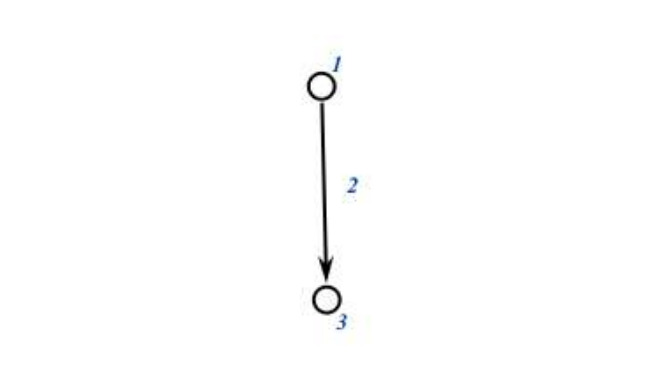
\includegraphics[scale=0.6]{Figure 1.png}
\caption\small{Example of three-element sc-construction}
 \label{fig:image1}
\end{figure}
\vspace{-8pt}

\begin{figure}[h!]
    \centering
    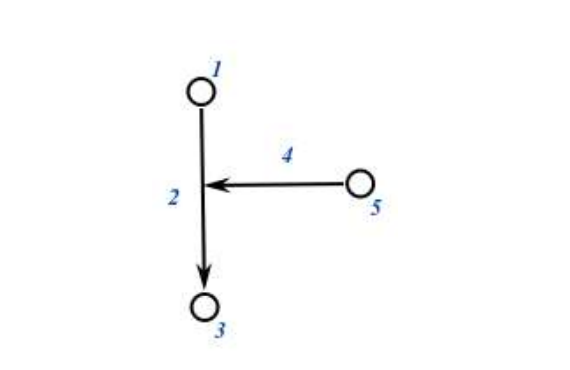
\includegraphics[scale=0.6]{Figure 2.png}
    \caption{\small Example of five-element sc-construction}
    \label{fig:image2}
\end{figure}

The \textit{software interface} of these\textit{ methods} is constrained
by the \textit{method representation language C++}. For example,
using these\textit{ methods} you cannot create\textit{ iterators} by
specifying only \textit{sc-memory element classes$\Hat{}$} as arguments,
by which you need to find all \textit{corresponding constructions
in sc-memory} , where \textit{classes of their sc-storage$\Hat{}$} are the
classes passed as arguments to the specified methods,
nor is it possible to specify as arguments anything other \qquad

\noindent than an \textit{sc-address} or an \textit{sc-memory element class$\Hat{}$}. An
attempt to perform any of the above will result in an
error of "gluing" the interface of one of the specified
\textit{methods} specified in the \textit{C++} header file with the
implementation with the specified parameters specified
in the C++ source file because the C++ compiler cannot
find an implementation for the specified \textit{software interface}.
Thus, due to the aforementioned problem, the parameters
for\textit{ Method for creating a three-element sc-memory
construction search iterator} and\textit{ Method for creating a
five-element sc-memory construction search iterator} can
be \textit{sc-address} and/or \textit{sc-memory element class$\Hat{}$}.
The \textit{iterators} created using the specified \textit{methods} also
have a \textit{software interface}. The results of both \textit{methods}
are different \textit{iterators}, that share, however, the same
\textit{software interface}. Such \textit{iterators} allow you to work
with \textit{sc-memory constructions} at the same moment they
are found. Using the\textit{ Method of moving to the next scmemory construction "suitable" for the specified iterator},
the\textit{ iterator} updates its internal state each time a new
sc-memory construction is found. By next \textit{sc-memory
construction "suitable" for the specified iterator} we
mean an \textit{sc-memory construction} whose elements match
the configuration of the created \textit{sc-memory construction
search iterator} and which was not found earlier.r. The result
of the latter\textit{ method} is the boolean \textit{True} value if the next
"suitable" construction for the specified \textit{iterator }exists in
\textit{sc-memory}. If there are no "suitable" constructions for this
\textit{iterator} in\textit{ sc-memory}, then the \textit{Method of moving to the
next sc-memory construction "suitable" for the specified
iterator} results in the boolean value \textit{False}. To get the \textit{sc-address} of some of the elements of the found \textit{sc-memory construction}, you must use the \textit{Method of accessing the sc-address of the specified sc-memory construction element} by the position number of this element in the specified
sc-memory construction, specifying as an argument an
integer value in the form of the position index of the
searched element in this construction. In this case, the
indexing of the positions of elements in the\textit{ sc-memory
construction} in the current \textit{Implementation of sc-memory
in the ostis-platform} starts from zero, not from one, and
the indexing order is determined by the order of arguments
that have been used when creating the \textit{iterator}. If you
try to specify for this method an index for which there is
no position in this construction, this method will result
in an invalid element position in the specified\textit{ sc-memory
construction exception}. Thus, the range of indices for
\textit{three-element constructions} is limited from zero to two,
and for five-element constructions, from zero to four. 

\noindent \textbf{\textit{S\,o\,f\,t\,w\,a\,r\,e i\,n\,t\,e\,r\,f\,a\,c\,e f\,o\,r i\,n\,f\,o\,r\,m\,a\,t\,i\,o\,n\\
r\,e\,t\,r\,i\,e\,v\,a\,l m\,e\,t\,h\,o\,d\,s o\,f
I\,m\,p\,l\,e\,m\,e\,n\,t\,a\,t\,i\,o\,n o\,f
s\,c-m\,e\,m\,o\,r\,y i\,n t\,h\,e o\,s\,t\,i\,s-p\,l\,a\,t\,f\,o\,r\,m\\}}

\begin{level1}
 \item[\textbf{$\supset=$} ]
 \item[\textbf{\}}] 
  \item[\textbf{$\supset$} ] \textit{Extension of Software interface for information}
\end{level1}


\href{https://ru.wikipedia.org/wiki/%D0%90%D1%80%D0%B1%D1%83%D0%B7}{[27]}




\end{document}
  